% Options for packages loaded elsewhere
\PassOptionsToPackage{unicode}{hyperref}
\PassOptionsToPackage{hyphens}{url}
\PassOptionsToPackage{dvipsnames,svgnames,x11names}{xcolor}
%
\documentclass[
  10pt,
]{article}

\usepackage{amsmath,amssymb}
\usepackage{iftex}
\ifPDFTeX
  \usepackage[T1]{fontenc}
  \usepackage[utf8]{inputenc}
  \usepackage{textcomp} % provide euro and other symbols
\else % if luatex or xetex
  \usepackage{unicode-math}
  \defaultfontfeatures{Scale=MatchLowercase}
  \defaultfontfeatures[\rmfamily]{Ligatures=TeX,Scale=1}
\fi
\usepackage{lmodern}
\ifPDFTeX\else  
    % xetex/luatex font selection
\fi
% Use upquote if available, for straight quotes in verbatim environments
\IfFileExists{upquote.sty}{\usepackage{upquote}}{}
\IfFileExists{microtype.sty}{% use microtype if available
  \usepackage[]{microtype}
  \UseMicrotypeSet[protrusion]{basicmath} % disable protrusion for tt fonts
}{}
\makeatletter
\@ifundefined{KOMAClassName}{% if non-KOMA class
  \IfFileExists{parskip.sty}{%
    \usepackage{parskip}
  }{% else
    \setlength{\parindent}{0pt}
    \setlength{\parskip}{6pt plus 2pt minus 1pt}}
}{% if KOMA class
  \KOMAoptions{parskip=half}}
\makeatother
\usepackage{xcolor}
\setlength{\emergencystretch}{3em} % prevent overfull lines
\setcounter{secnumdepth}{-\maxdimen} % remove section numbering
% Make \paragraph and \subparagraph free-standing
\makeatletter
\ifx\paragraph\undefined\else
  \let\oldparagraph\paragraph
  \renewcommand{\paragraph}{
    \@ifstar
      \xxxParagraphStar
      \xxxParagraphNoStar
  }
  \newcommand{\xxxParagraphStar}[1]{\oldparagraph*{#1}\mbox{}}
  \newcommand{\xxxParagraphNoStar}[1]{\oldparagraph{#1}\mbox{}}
\fi
\ifx\subparagraph\undefined\else
  \let\oldsubparagraph\subparagraph
  \renewcommand{\subparagraph}{
    \@ifstar
      \xxxSubParagraphStar
      \xxxSubParagraphNoStar
  }
  \newcommand{\xxxSubParagraphStar}[1]{\oldsubparagraph*{#1}\mbox{}}
  \newcommand{\xxxSubParagraphNoStar}[1]{\oldsubparagraph{#1}\mbox{}}
\fi
\makeatother


\providecommand{\tightlist}{%
  \setlength{\itemsep}{0pt}\setlength{\parskip}{0pt}}\usepackage{longtable,booktabs,array}
\usepackage{calc} % for calculating minipage widths
% Correct order of tables after \paragraph or \subparagraph
\usepackage{etoolbox}
\makeatletter
\patchcmd\longtable{\par}{\if@noskipsec\mbox{}\fi\par}{}{}
\makeatother
% Allow footnotes in longtable head/foot
\IfFileExists{footnotehyper.sty}{\usepackage{footnotehyper}}{\usepackage{footnote}}
\makesavenoteenv{longtable}
\usepackage{graphicx}
\makeatletter
\newsavebox\pandoc@box
\newcommand*\pandocbounded[1]{% scales image to fit in text height/width
  \sbox\pandoc@box{#1}%
  \Gscale@div\@tempa{\textheight}{\dimexpr\ht\pandoc@box+\dp\pandoc@box\relax}%
  \Gscale@div\@tempb{\linewidth}{\wd\pandoc@box}%
  \ifdim\@tempb\p@<\@tempa\p@\let\@tempa\@tempb\fi% select the smaller of both
  \ifdim\@tempa\p@<\p@\scalebox{\@tempa}{\usebox\pandoc@box}%
  \else\usebox{\pandoc@box}%
  \fi%
}
% Set default figure placement to htbp
\def\fps@figure{htbp}
\makeatother

\makeatletter
\@ifpackageloaded{caption}{}{\usepackage{caption}}
\AtBeginDocument{%
\ifdefined\contentsname
  \renewcommand*\contentsname{Table of contents}
\else
  \newcommand\contentsname{Table of contents}
\fi
\ifdefined\listfigurename
  \renewcommand*\listfigurename{List of Figures}
\else
  \newcommand\listfigurename{List of Figures}
\fi
\ifdefined\listtablename
  \renewcommand*\listtablename{List of Tables}
\else
  \newcommand\listtablename{List of Tables}
\fi
\ifdefined\figurename
  \renewcommand*\figurename{Figure}
\else
  \newcommand\figurename{Figure}
\fi
\ifdefined\tablename
  \renewcommand*\tablename{Table}
\else
  \newcommand\tablename{Table}
\fi
}
\@ifpackageloaded{float}{}{\usepackage{float}}
\floatstyle{ruled}
\@ifundefined{c@chapter}{\newfloat{codelisting}{h}{lop}}{\newfloat{codelisting}{h}{lop}[chapter]}
\floatname{codelisting}{Listing}
\newcommand*\listoflistings{\listof{codelisting}{List of Listings}}
\makeatother
\makeatletter
\makeatother
\makeatletter
\@ifpackageloaded{caption}{}{\usepackage{caption}}
\@ifpackageloaded{subcaption}{}{\usepackage{subcaption}}
\makeatother

\usepackage{bookmark}

\IfFileExists{xurl.sty}{\usepackage{xurl}}{} % add URL line breaks if available
\urlstyle{same} % disable monospaced font for URLs
\hypersetup{
  pdftitle={Credit Score Classification -- EDA \& Project Plan},
  colorlinks=true,
  linkcolor={blue},
  filecolor={Maroon},
  citecolor={Blue},
  urlcolor={Blue},
  pdfcreator={LaTeX via pandoc}}


\title{Credit Score Classification -- EDA \& Project Plan}
\author{}
\date{}

\begin{document}
\maketitle


\section{🧩 Problem Definition}\label{problem-definition}

This is a multi-class \textbf{classification problem} to predict
\texttt{Credit\_Score} (Poor, Standard, Good) based on user demographic
and financial behavior data. The dataset contains \textasciitilde100,000
records and was sourced from Kaggle.

\subsection{Why this problem is
interesting}\label{why-this-problem-is-interesting}

\begin{itemize}
\tightlist
\item
  Real-world financial risk prediction\\
\item
  Dataset includes missing values, noise, imbalance\\
\item
  Useful for supervised classification techniques
\end{itemize}

\section{🗃️ Dataset Overview}\label{dataset-overview}

\begin{itemize}
\tightlist
\item
  \textbf{Samples:} \textasciitilde100,000\\
\item
  \textbf{Features:} mix of numeric and categorical\\
\item
  \textbf{Target:} \texttt{Credit\_Score} (Poor, Standard, Good)\\
\item
  \textbf{Challenges:} outliers, noisy values (\texttt{\_\_\_\_\_\_\_},
  symbols), imbalance
\end{itemize}

\section{🔍 Missing Value Assessment}\label{missing-value-assessment}

\begin{verbatim}
                      ID              Customer_ID                    Month 
                       0                        0                        0 
                    Name                      Age                      SSN 
                       0                        0                        0 
              Occupation            Annual_Income    Monthly_Inhand_Salary 
                       0                        0                    15002 
       Num_Bank_Accounts          Num_Credit_Card            Interest_Rate 
                       0                        0                        0 
             Num_of_Loan             Type_of_Loan      Delay_from_due_date 
                       0                        0                        0 
  Num_of_Delayed_Payment     Changed_Credit_Limit     Num_Credit_Inquiries 
                       0                        0                     1965 
              Credit_Mix         Outstanding_Debt Credit_Utilization_Ratio 
                       0                        0                        0 
      Credit_History_Age    Payment_of_Min_Amount      Total_EMI_per_month 
                    9030                        0                        0 
 Amount_invested_monthly        Payment_Behaviour          Monthly_Balance 
                       0                        0                        0 
            Credit_Score 
                       0 
\end{verbatim}

\pandocbounded{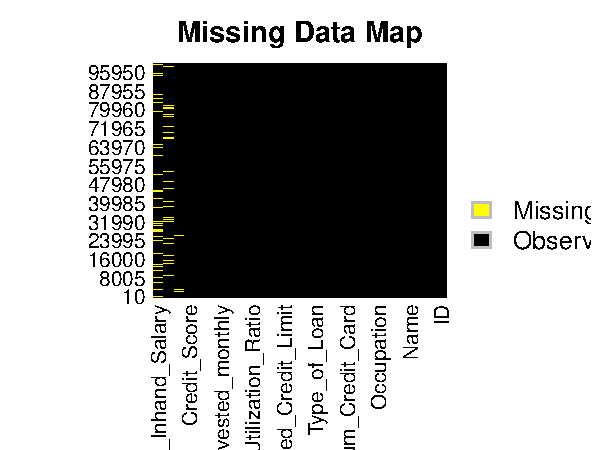
\includegraphics[keepaspectratio]{Final_Report_3Page_HTML_Folded_files/figure-pdf/unnamed-chunk-3-1.pdf}}

\textbf{Summary:} \textasciitilde1\% missing. Most common:
\texttt{Credit\_History\_Age}, \texttt{Monthly\_Inhand\_Salary},
\texttt{Amount\_invested\_monthly}

\section{🧹 Data Cleaning and Type
Fixes}\label{data-cleaning-and-type-fixes}

\section{📊 Target Class Distribution}\label{target-class-distribution}

\pandocbounded{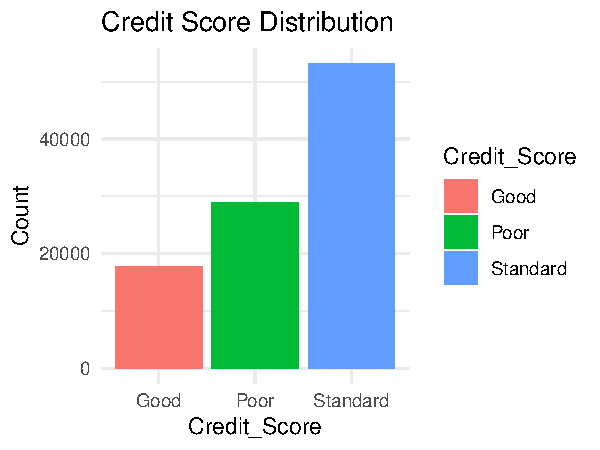
\includegraphics[keepaspectratio]{Final_Report_3Page_HTML_Folded_files/figure-pdf/unnamed-chunk-5-1.pdf}}

\section{🧭 Outlier Detection}\label{outlier-detection}

\pandocbounded{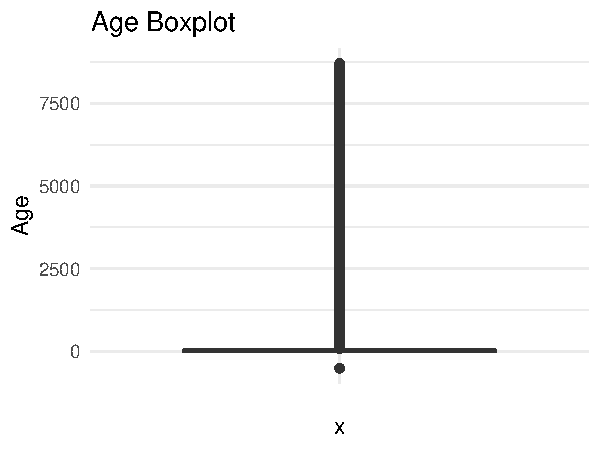
\includegraphics[keepaspectratio]{Final_Report_3Page_HTML_Folded_files/figure-pdf/unnamed-chunk-6-1.pdf}}

\section{🧮 Correlation and PCA}\label{correlation-and-pca}

\subsection{Correlation Matrix (Simplified for
Clarity)}\label{correlation-matrix-simplified-for-clarity}

\pandocbounded{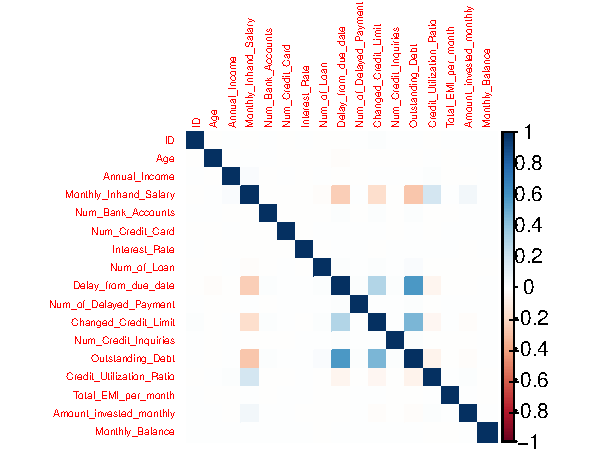
\includegraphics[keepaspectratio]{Final_Report_3Page_HTML_Folded_files/figure-pdf/unnamed-chunk-7-1.pdf}}

\subsection{PCA Plot}\label{pca-plot}

\pandocbounded{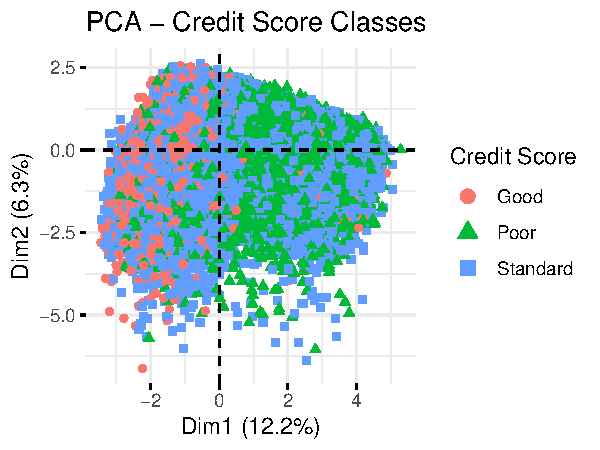
\includegraphics[keepaspectratio]{Final_Report_3Page_HTML_Folded_files/figure-pdf/unnamed-chunk-8-1.pdf}}

\section{🧭 Project Plan}\label{project-plan}

\subsection{📅 Phase Overview}\label{phase-overview}

\begin{itemize}
\tightlist
\item
  Phase 1: Cleaning \& Feature Prep\\
\item
  Phase 2: EDA \& Visuals\\
\item
  Phase 3: Modeling (Logistic, Tree, RF, XGBoost)\\
\item
  Phase 4: Evaluation\\
\item
  Phase 5: Predictions\\
\item
  Phase 6: Reporting
\end{itemize}

\subsection{📆 Weekly Timeline with
Subtasks}\label{weekly-timeline-with-subtasks}

\begin{longtable}[]{@{}
  >{\raggedright\arraybackslash}p{(\linewidth - 2\tabcolsep) * \real{0.4615}}
  >{\raggedright\arraybackslash}p{(\linewidth - 2\tabcolsep) * \real{0.5385}}@{}}
\toprule\noalign{}
\begin{minipage}[b]{\linewidth}\raggedright
Week
\end{minipage} & \begin{minipage}[b]{\linewidth}\raggedright
Tasks
\end{minipage} \\
\midrule\noalign{}
\endhead
\bottomrule\noalign{}
\endlastfoot
\textbf{1} & - Remove invalid values - Impute missing - Fix placeholders
- Encode categorical vars \\
\textbf{2} & - Class imbalance plots - Outlier checks - Correlation -
PCA \\
\textbf{3} & - Train models - Tune \& evaluate using F1, Confusion
Matrix \\
\textbf{4} & - Predict \& export - Finalize report - Present findings \\
\end{longtable}

\subsection{📈 Gantt Chart}\label{gantt-chart}

\begin{figure}[H]

{\centering \pandocbounded{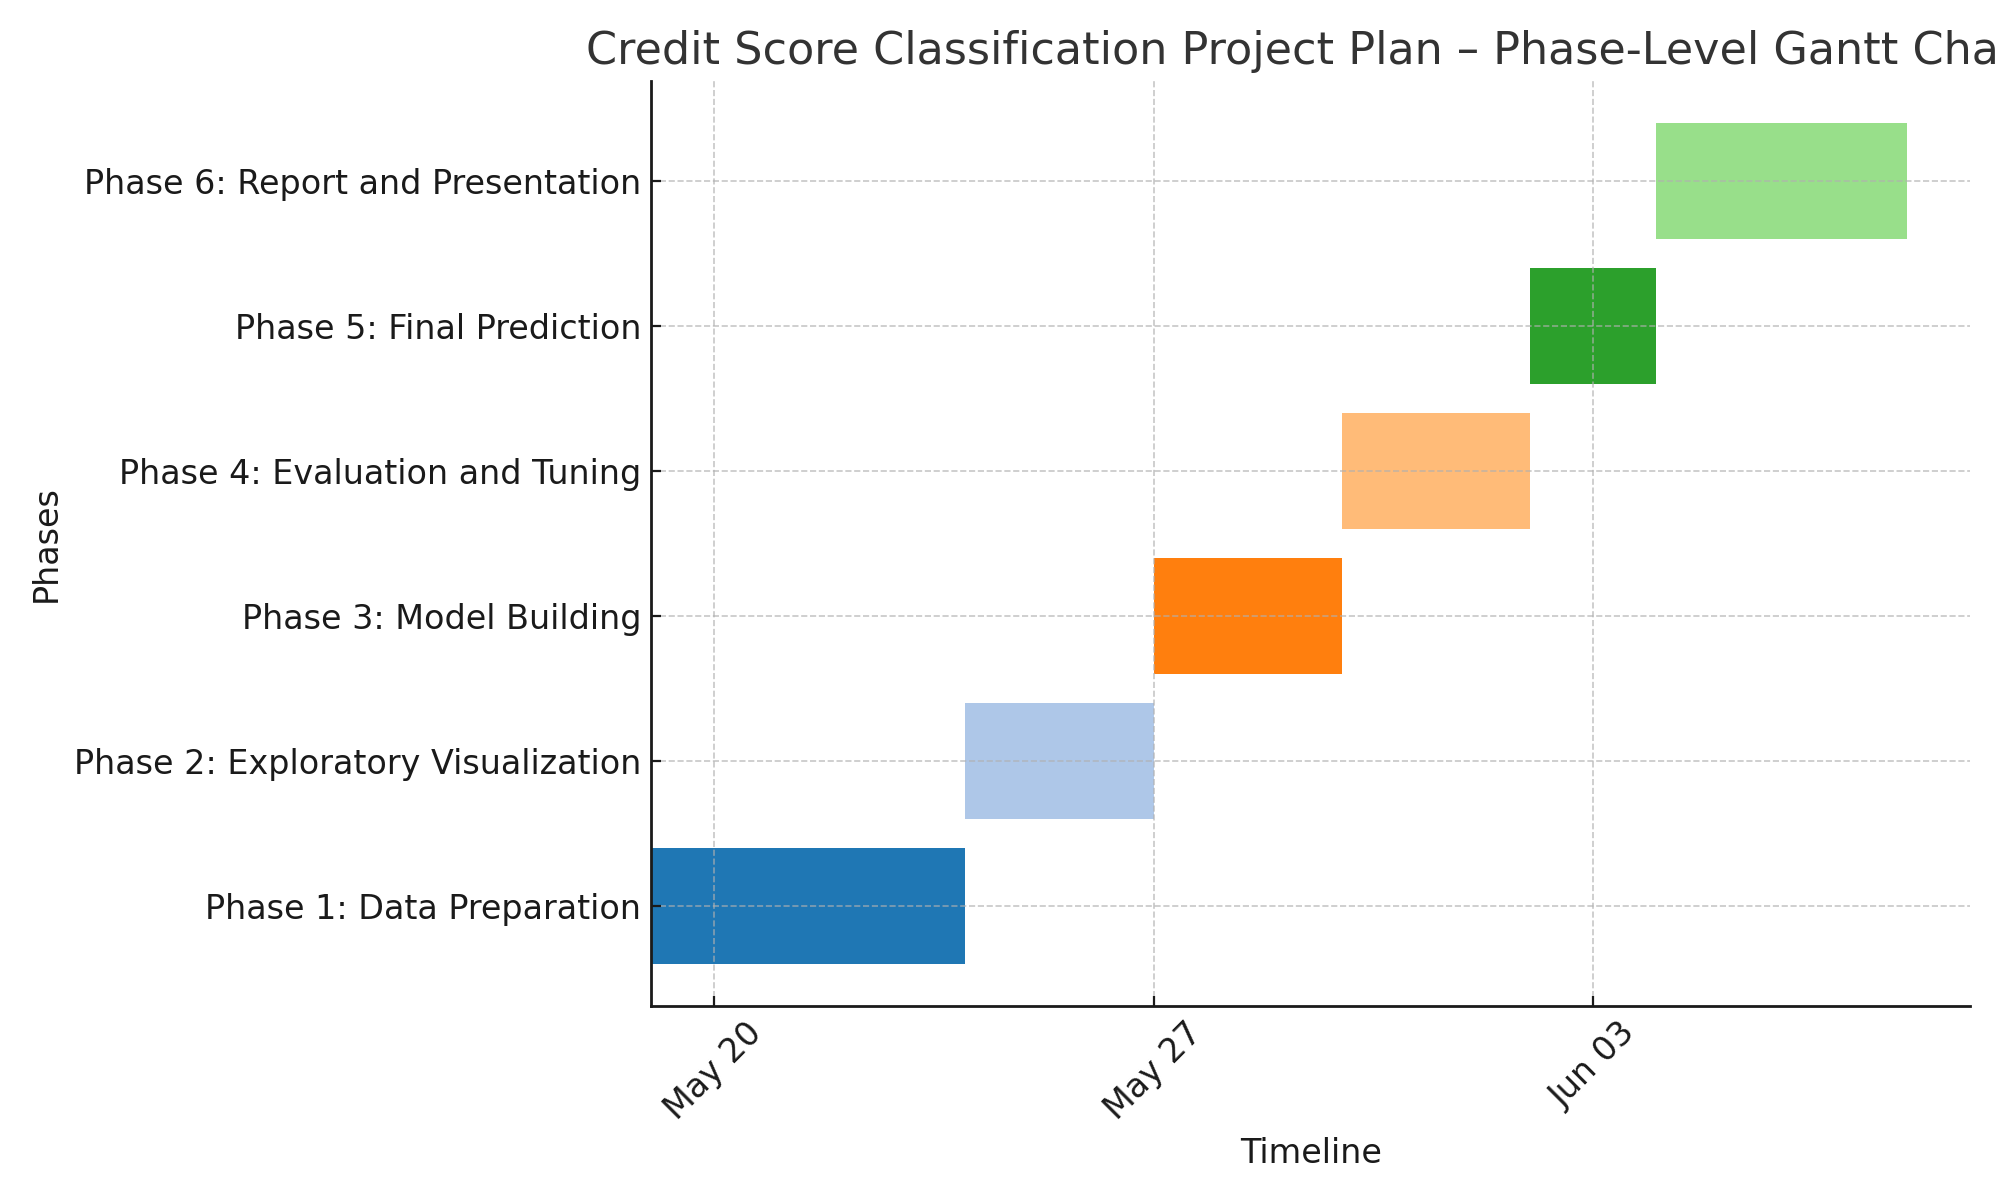
\includegraphics[keepaspectratio]{project_gantt_phases_only.png}}

}

\caption{Gantt Chart}

\end{figure}%

\section{📏 Evaluation Metrics}\label{evaluation-metrics}

\begin{itemize}
\tightlist
\item
  Macro \textbf{F1-score}\\
\item
  Class-wise \textbf{precision}, \textbf{recall}\\
\item
  Confusion Matrix for multi-class performance
\end{itemize}

\section{✅ Summary}\label{summary}

This project plan and EDA establish a clean foundation for multi-class
classification. Techniques include PCA, correlation analysis, and
strategies for model evaluation and improvement.




\end{document}
